\section{Introduction}

%Exploratory data analytics (EDA) is a technique where analysts or data scientists attempt to understand the inherent characteristics of data and get interesting insights.
%from a new dataset or an existing dataset that is periodically being updated.
Exploratory data analysis (EDA) is an interactive and sequential process of data understanding and insight generation where a user (e.g. a data analyst) issues an analysis action (i.e. a query) against a tabular data, receives some answers, subsection of the tabular data or some visualization and then decides which queries to issue next in order to understand the hidden characteristics of the data and associated insights better~\cite{ma2021metainsight, atena2020sigmod, edasim2018kdd}.
Characteristics and insights obtained using EDA are crucial for subsequent decision making in various domains~\cite{ma2021metainsight}.
%
\begin{comment}
\noindent\textbf{Intent.}
Each of the EDA sessions corresponding to a sequence of interactions with the data, has an underlying \textit{intent} that often remains implicit to even the user until they arrive at some interesting characteristics and then follow some intuitions to find an insight.
For example: an analyst started exploring flights arrival/departure related data, noticed unusually high delay in a month for some airline and then focused to understand the root-cause. Another example: an analyst started exploring number of airlines operating from different airports and their delay patterns. But ultimately arrived at some insight about which two pair of airlines have worse connecting flight timing coordination. 
Note: none of these intents are known apriori and also does not get explicitly labeled afterwards.  
\end{comment}
%
The \textit{success} of an EDA session and the quality of insights obtained from it large depend on two things: (1) how interactive the system is (i.e. how quickly results are obtained) and (2) whether the outcome of previous sequence of queries are reliable and representative enough for an expert analyst to issue subsequent queries so as to uncover interesting characteristics. 
%
\begin{comment}
%
Several studies have shown that high interaction latency can drastically degrades the quality of insights due to mental fatigue and loss of continuity in the mental thought process~\cite{liu2014effects, moritz2017trust}. 
\end{comment}
%
\begin{figure}[t]
\begin{center}
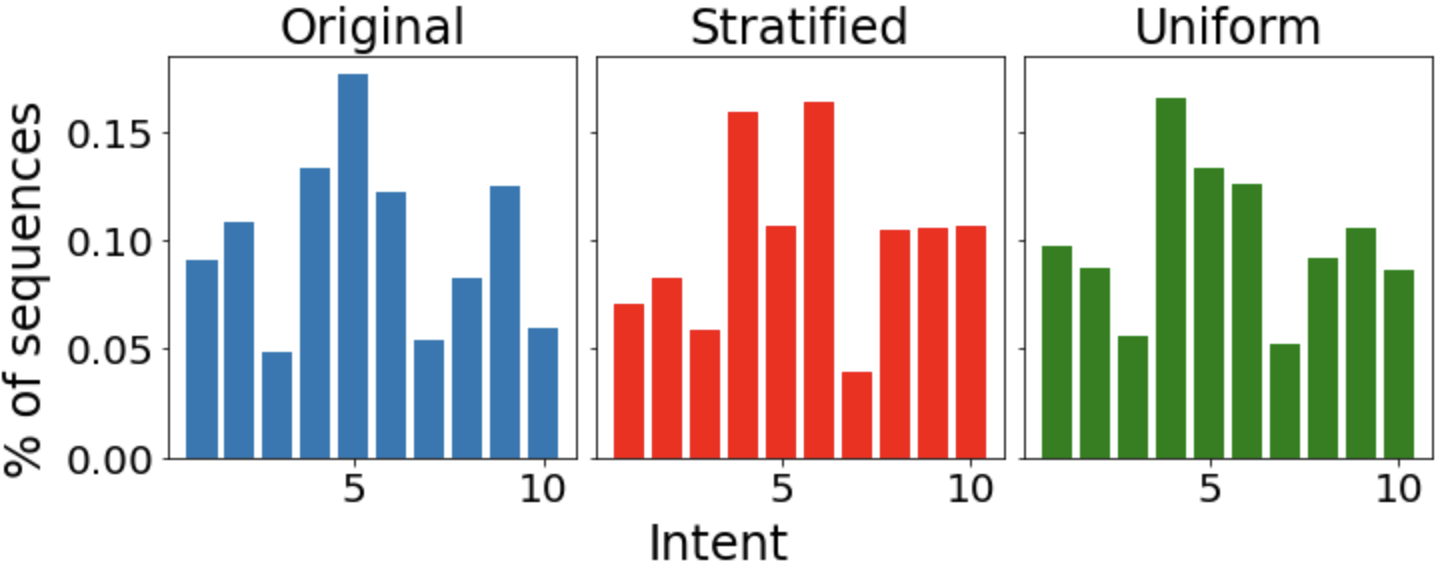
\includegraphics[width=0.85\columnwidth, height=0.25\columnwidth]{LaTeX/figures/intent_skew.png}
     \caption{Divergence of intent distribution: Single sampling strategy (stratified or uniform) for all the contexts in sequential data exploration can make user to get mislead into wrong analysis flow due to approximation errors.} 
     \label{fig:intent_skew}
\end{center}
\end{figure}

%Need for approximations
To improve latency of interactions, downsampling the data has been proposed in various works target ting approximate query processing (AQP)~\cite{chaudhuri2017approximate, park2018verdictdb, sheoran2022aaai} and visualizations~\cite{park2016visualization, moritz2017trust, porwal2022sigmod}. For large datasets that are often a target for EDA~\cite{galakatos2017revisiting, wang2014sample}, running queries on samples can substantially reduce the query latency.
%Transparency is a desirable property here because, burdening the user with another information about approximation error would make the already cumbersome EDA process even more complex. Studies have shown that users are poor at making their decisions based on approximation errors (CHI-2018).
However, sampling creates approximation errors and can mislead the users in an interactive data exploration flow, especially when the use, choice and degree of approximation is transparent to the user.
In this paper we are the first to explore a setting where an EDA system \textit{transparently} uses different forms of downsampling strategy on the original data to run the queries but protect the user from being mislead due to approximation error from poor choice of samples. 
%
Figure~\ref{fig:intent_skew} shows distributions of 10 user-intents extracted from several thousand of realistic EDA sequences on Flights data.
%using EDA simulator that can generate realistic analyses patterns similar expert users with various implicit intents~\cite{atena2020sigmod}.
It can be observed that if only a particular downsample strategy (e.g. stratified or uniform sampling) is used for every context in the entire sequence, the resulting intent distribution diverges from the ideal. 
% This indicates that blindly using any such samples can mislead the analysts.  
%
%as they often choose the next sequence of query based on display from the previous results. 
%
This is because the results of the previous query can get distorted due to sampling and may prompt the user to a false path of analysis, which would have been useless if the original data was used. Second, there are numerous sampling techniques available, such as uniform sampling with different sampling rates, stratified sampling of few different kinds, systematic sampling, cluster sampling, diversity sampling etc.
%
%
Each of these sampling algorithms are good at preserving some properties of the data at the cost of introducing approximation errors for other properties. 
%The best sampling method that can minimize the approximation error often depends on the particular structure of the query and the underlying data distribution. 
For a sequential and interactive data exploration workflow where multiple different types of queries are used on different subsections of the data, there is often not a single sampling strategy that wins over everything else. This is because, in a sequential interactive exploration the amount of approximation in the results or visualizations generated from the previous queries, influences the user decision on what next query to run. 
%Greedy solution that would pick the sample that produces lowest approximation error for the next query, is also infeasible.
%This is because actual approximation errors can not be calculated without running the query against each of the samples which can be prohibitively expensive for an interactive setting. 
Moreover, there is a trade-off between query latency and accuracy, when sampling is used.
Choosing a sample that gives higher approximation error (while making the query faster) can be desirable, as long as the approximation error does not mislead the user to make wrong decisions about subsequent analyses flow or alter the key takeaways.  

This brings us to the second major problem that we handle in this paper. EDA being fundamentally an open-ended and expertise-driven process to understand a new dataset, there is no explicit \emph{intent} that can be attributed to the analysis flow.
%For example: an analyst started exploring flights arrival/departure related data, noticed unusually high delay in a month for some airline and then focused to understand the root-cause. Another example: an analyst started exploring number of airlines operating from different airports and their delay patterns. But ultimately arrived at some insight about which two pair of airlines have worse connecting flight timing coordination. 
%Note: none of these intents are known apriori and also does not get explicitly labeled afterwards.  
Some recent papers looked at how to learn from EDA sequences performed by expert users in order to mimic those in a simulator to generate a sequence of queries and results on a new dataset, to help novice analysts~\cite{atena2020sigmod}.
Similarly~\cite{edasim2018kdd} provides suggestions to novice users about the next query to run based on learning from expert user sessions. 
While these works identify that exploratory analysis is not exactly random in nature and expert analysts usually follow few core implicit intents, but they do not handle how intent-aware learning can be performed in such situations. 
This lack of clear intent, as well as not having a clear measure of success or a implicit/explicit feedback at the end also makes our problem markedly distinct from other interactive settings such as task-oriented dialog systems \cite{liu2018dialogue,shi2019build}, conversational recommender systems \cite{lei2020interactive,zhang2020conversational} and interactive retrieval systems \cite{guo2018dialog}. When developing the learning agent for these systems, it is usually assumed that the users have a clear intent, from which the loss function or reward function can be naturally derived. However, in our task the users usually have implicit intent, which makes development of the reward function non-trivial. %\tong{As the first work focusing on approximate exploratory data analysis in an interactive setting, it is assumed that }
%interactions with a chat-bot on a particular task~\cite{}.
%\sm{Tong, can you please expand a bit? and add citations.}
%
%\sm{“The authors introduce a new concept of intent-divergence early on (ln 164), but however, never explain it in any detail. It remains unclear why the proposition prevents an intent-divergence of the user. If the analyst’s intent actually changes, preventing an intent divergence on the model side, seems to hinder their workflow.The manuscript does not include a discussion of the relevant problem of “intent-shift”.”}


To jointly address the above two challenges, we propose an intent-aware deep reinforcement learning (DRL) framework, \name, to enable the interactive exploratory data analysis in the presence of approximation errors. 
\begin{comment}
Specifically,
\begin{itemize}
        \item We down-sample the data at each time and optimize the down-sampling strategies over time, by modeling the strategies as actions in reinforcement learning.
        \item We develop a novel reward function via topic modelling to discover the user intention without labeled intention data.
        \item We develop a termination criteria to guide the model training in the sequential data exploration,
        by capturing key takeaway insights.
        This leads to more  sample-efficient intent-aware reinforcement learning.
\end{itemize}
\end{comment}
%
In this paper, we focus on how to prevent intent-divergence (\emph{i.e.}, approximation errors misleads users to a different intent). It is assumed that there is limited \textit{intent-shift} (\emph{i.e.}, change of user's core intent characteristics) in the problem setting. 
%While in this paper we are the first to address how to prevent intent-divergence (approximation errors misleads users to a different intent), 
This assumption is widely adopted in other interactive applications \cite{liu2018dialogue,guo2018dialog,tan2019drill}, although it is interesting to address the intent-shift \cite{xie2021tiage,arnold2019sector}. As the first work on approximate exploratory data analysis in the interactive setting, we leave addressing \textit{intent-shift} as future work.

\begin{comment}
subsection 1 (two datasets)
1\\
1 + 2\\
1 + 3\\
1 + 2 + 3\\

analysis:\\
subsection 2
a. different pool of down-sampling strategies to choose? corresponds to 1\\
subsection 3
b. number of cluster, 1+2+3
subsection 4
c. length of session, corresponds to 3, 1+2+3
\end{comment}

Our contributions are summarized as follows.
\begin{itemize}
    \item To our best knowledge, we are the first to identify an important yet practical problem where approximations should be used to improve interactivity in sequential exploration of data but can potentially mislead analysts to wrong analyses paths or intent-divergence. 
    \item We make a case that depending on the context of the sequential analysis, different sampling strategies would be optimal for providing lower interaction latency while protecting intent-divergence.   
    \item We novelly formulate the problem as a reinforcement learning task. Our formulation captures both the computational cost of executing the queries, as well as the sequential decisions made by users for different implicit intents. We model the choice of down-sampling strategy as the action-space and optimize the divergence of sequential interactions by an user along with the interactivity of the system, in the presence of approximations, in an intent-aware manner.
    To efficiently optimize the agent without explicit user intent, we develop a novel reward function and DRL learning stop criteria.
    \item We show the effectiveness of our technique by extensively evaluating our solution on 3 real-world datasets and against several baselines. 
    %Our method outperforms baselines in terms of intent preservation as well as latency, 
    We also present detailed ablation study and make our code and data available~\cite{open_repo}.
    
    %\item With extensive evaluations with 3 real world datasets, we show that ???...
    % \sm{Need results to be highlighted here.}
\end{itemize}

\begin{comment}
\tong{A potential flow: (please just ignore the parts which are not appropriate)
    \begin{enumerate}
        \item What is interactive exploratory data analysis? Why interactive is important.
        \item What are the challenges of developing interactive systems for exploratory data analytics? There are many existing interactive systems and applications, such as dialog system and interactive recommender system. Why developing interactive systems for exploratory data analytics is non-trival? What are the challenges?
        \begin{itemize}
            \item The computational cost is high, but the user desires real-time experience.
            \item The intent is not explicit or unclear. Thus, it is hard to develop the reward function.
            \item The intent is not explicit or unclear. Thus, it is hard to determine the termination of episode during training.
        \end{itemize}
        \item To jointly address the above challenges, we propose an intent-aware reinforcement learning framework to enable the interactive exploratory data analysis. Specifically,
        
        \begin{itemize}
        \item We downsample the data at each time and optimize the downsampling strategies over time, by modeling the strategies as actions in reinforcement learning.
        \item We develop a novel reward function via topic modelling to discover the user intention without labeled intention data.
        \item We develop a novel stop criteria to guide the model training and achieve sample-efficient reinforcement learning.
        \end{itemize}
        
        \item Our contributions are summarized as follows.
        \begin{itemize}
            \item We identify an important yet practical problem. We present the first work of ???.
            \item We novelly formulate the problem as a reinforcement learning task. To reduce the compuational cost, we model ??? as actions and optimize ??? over time. To efficiently optimize the agent without explict user intent, we devevelop a novel reward function and RL learning stop criteria.
            \item With extensive evaluations, we show that ???.
        \end{itemize}
        
    
    \end{enumerate}
}
\end{comment}


